\chapter{Life insurance cash flow model}
\label{chap:licfm}

The "Life insurance PillarOne cash flow model" is yet another of the public available models for \RA . It allows modeling the needs of a life insurance office with respect to a portfolio of unit-linked life insurance contracts (policies) and a traditional financing life reinsurance treaty.

The major objective is to model the future cash flows for a life insurance company for pricing (profit testing), valuation and planning purposes (incl.~embedded value calculations). The cash flows for the various stakeholders (policyholders, distribution channels, expenses, funds management, reinsurance, taxes, etc.) are calculated.

This chapter describes the functionalities of the PillarOne life insurance cash flow model from an end-user perspective. Throughout the chapter a concrete example is used to describe and illustrate the parameters, functionalities and results derived with \RA .

With this open life insurance model, the  following parameters can be described: 
\begin{itemize}
	\item Actual expenses (both company and product-based), 
	\item reinsurance conditions, 
	\item actual model points (existing portfolio) and future business, 
	\item product parameters/characteristics, 
	\item demographic assumptions (mortality, disability, lapses),
	\item economic and solvency assumptions, 
	\item distribution channel commissions, and 
	\item banking expenses.
\end{itemize}

Looking forward, \RA is also enable to implement useful stochastic calculations for life insurance in an open available model.

\section{Introduction}

Based on the existing PillarOne software an extension (so-called "Life insurance PillarOne cash flow model") has been built to model the needs of a life insurance office with a portfolio of unit-linked life insurance contracts (policies) and a traditional financing life reinsurance treaty. 

To model the life insurance cash flows with the various stakeholders the following elements need to be considered, as illustrated in figure \ref{fig:lifehighlevel}.

\begin{figure}[ht]
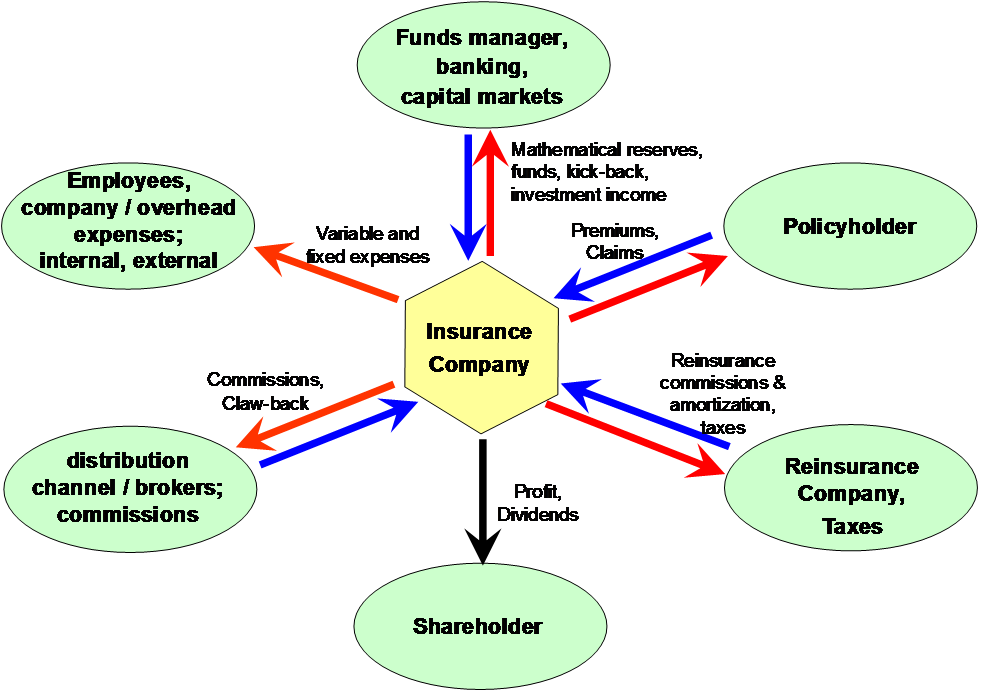
\includegraphics[scale=0.7]{images/lifehighlevel.png}
	\caption{Stakeholders' view of Life Insurance}
	\label{fig:lifehighlevel}
\end{figure}


At the very beginning there was a concrete project with the need to perform future cash flow projections of a life insurance company for pricing (profit testing), valuation and planning purposes (incl.~embedded value calculations). The life insurance PillarOne application has then been developed with the following main objectives:

\begin{itemize}
	\item Perform cash flow projections on a shorter (e.g.~3 years for planning purposes) as well as a longer (e.g.~20 years for embedded and appraisal value calculations) term horizon
	\item Consider an existing portfolio as well as model future new business
	\item Determine the shareholders' profitability for the modeled business
	\item Appropriately consider and analyze the reinsurance treaty (e.g.~costs of financing, pay-back period)
	\item Apply profit testing techniques on life insurance products and analyzing LoBs
\end{itemize}

The components of the PillarOne life insurance calculations and workflow can be characterized with chart \ref{fig:lifeworkflow}.

\begin{figure}
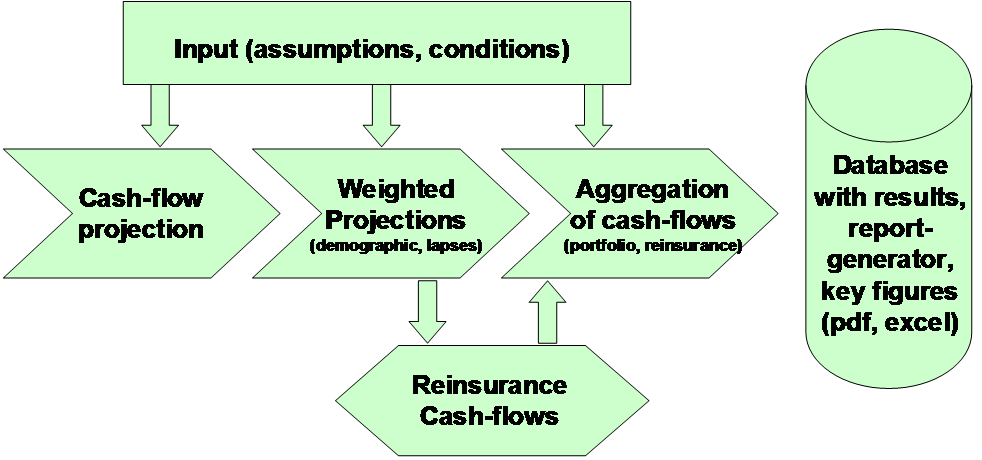
\includegraphics[scale=0.7]{images/lifeworkflow.png}
	\caption{Life Insurance Workflow Calculations and Workflow}
	\label{fig:lifeworkflow}
\end{figure}

The building blocks are:

\begin{itemize}
	\item Cash flow projection calculation engine for a simple life insurance policy
	\item Weighted by actual demographic and lapse experiences
	\item Aggregation on all policies on entire portfolio
	\item Consideration of reinsurance cash flows
	\item Storage of results in a database enabling to derive all kind of statistics (report-generator, key figures): EV and VIF, new business margin, IRR, break-even analysis before/after reinsurance, perform planning with future new business, sensitivities, etc.
	\item Consideration of an entire range of assumptions and conditions.
\end{itemize}

This chapter describes the functionalities of the PillarOne life insurance cash flow model from an end-user perspective. Throughout the chapter a concrete example is used to describe and illustrate the parameters, functionalities and results derived with the software. The GUI (graphic user interface) enables to enter a whole range of assumptions and conditions. With a well structured and modular end-user interface all the necessary input parameters can be captured.

This chapter of the manual is structured in the following way:
\begin{itemize}
	\item In the next section \ref{sec:lifeexample} the (high-level) framework of the used example is presented.
	\item In subsequent sections the input, calculations and results/output are described in detail.
	\item At the end, in section \ref{sec:lifeoutlook}, we will deal with potential future development of this life insurance PillarOne cash flow model.
\end{itemize}

This documentation is based on an illustrative example which includes the (direct) life insurance (a company with a portfolio of unit-linked policies) with an associated reinsurance treaty. If there is no interest in the reinsurance section, one could simply exclude the reinsurance by setting the quota share reinsurance parameters to 0. All the calculations and results are done and derived on a deterministic basis. 

Please note: The example in this documentation should only be seen as an illustration. In other words: The parameters, content and result of this example cannot directly be used in the practical work without considering further input reflecting the company specific characteristics, concrete products, appropriate demographic and economic environment, etc.

\section{Example}\label{sec:lifeexample}

When downloading and installing \RA{} you directly get a preinstalled life example. In this chapter, we will discuss this example at length. We provide illustrative numbers only and you are free to change whatever you want. 

\subsection{Product characteristics}
We will model three unit-linked products: Two periodic premium products which are designed for different commission payments (com5 and com4 for e.g.~different distribution channels) and a single premium product. We will denominate the products with ULPPCOM5, ULPPCOM4 and ULSPCOM5. We will work only in CHF. However, the life model would also allow capturing segregated currency-pots to reflect different currencies by converting the data into CHF.

From the gross premium (premium paid by the policyholder) the expenses and charges are deducted. The remaining saving premium is then added to the actual funds value (saving or funds accumulation process). To describe the actual products (so-called pricing or "1st order" basis) we use the following parameters for the expense and cost structure:
\begin{itemize}
	\item Acquisition expenses (alpha): 5\% of the present values of the paid premiums, which are amortized over the first 10 policy years
	\item Collection expenses (beta): between 7\% and 8\% of the periodic premium
	\item Proportional administration expenses (gamma): 0.05\% (for periodic premiums) or 0.25\% (for single premium) p.a.~of the funds value
	\item Fixed administration expenses (kappa): between CHF 50 to CHF 100 per policy p.a.~
	\item Costs for mortality risk premium: Monthly calculated according to the sum at risk in case of death and the pricing mortality table according to age and gender of the policyholder
	\item Costs for waiver of premium: Monthly calculated according to the sum at risk in case of disability and the pricing waiver of premium table according to waiting period, age and gender of the policyholder
	\item Surrender charges: For the periodic premium products 100\% of the funds value linearly falling to 0\% of the funds value over the first 5 policy years.
\end{itemize}

The following risk benefits could be defined and set at policy level:
\begin{itemize}
	\item Sum at risk in case of death could be defined as:
		\begin{itemize}
			\item	a fixed CHF-amount less the actual funds value and/or as
			\item a percentage of the sum of the paid premiums.
		\end{itemize}
	\item Waiver of premiums for the periodic premiums with various waiting periods (e.g.~6, 12 or 24 months).
\end{itemize}

The expense loadings and costs are either deducted from the (periodic) premium payments or from the funds of the policy. Similarly the mortality and disability costs ("1st order" risk premiums according to mortality and waiver of premium tables) are periodically deducted. The calculations are done on a monthly basis.

\subsection{Distribution channel commissions}
There are two commission payment types or "scales" (COM5 and COM4): Either 5\% or 4\% of the sum of premiums (total paid premiums over the entire policy duration, but the policy duration will be capped at a maximum of 25 years). The commissions are paid upfront. However, in case of policy surrender they have to be refunded ("claw-back") by the distribution channel (agent) linearly, in proportion within the first three policy years; i.e.~ only after three years the commissions are fully earned. A general shortfall of the claw-back payment of 2.5\% is assumed.
Finally, a portfolio commission of 0.05\% p.a.~ of the mathematical reserves (funds value) will be paid out on a monthly basis.

\subsection{Actual expenses}
The actual expenses ("2nd order" parameters) could be defined on a company basis and/or on a product-related basis. In addition the expenses could also be linked to inflation. In our example we do not assume total company expenses (no expense over-run). We have actual initial expenses between CHF 200 and CHF 350 per policy. The actual administration expenses are varying between CHF 150 and CHF 225 p.a.~ The expenses are depending on the policy size (sum of total paid premiums).

\subsection{Actual demographic assumptions}
For the actual mortality ("2nd order") various, product-related probability tables could be defined and used. Similarly for the disability (waiver of premium) and the lapses actual probability tables are assumed in the example. In our example the actual mortality and disability probability rates are 80\% of the pricing assumptions.

\subsection{Reinsurance section}
According to the reinsurance treaty conditions, common or general reinsurance parameters need to be defined for all the products:
\begin{itemize}
	\item Various settlement dates and intervals
	\item Deposit interest rate of 0.25\% and reinsurance profit participation of 90\%
	\item Loss carried forward for all past underwriting years (amounts and interest rates) and for various currencies separately
	\item Reinsurance claw-back percentage of 100\% and 'cost and risk annual supplement on ceded premium' of 2\%, etc.
\end{itemize}

Product specific reinsurance parameters - which need to be entered - are:

\begin{itemize}
	\item The currency (CHF) and reinsurance quota share percentage of 50\%
	\item Reinsurance acquisition commission of either 5\% or 4\% of the sum of the reinsured premiums (total paid premiums to reinsurance company over the entire policy duration). However, the policy duration will be capped at a maximum of 25 years. We will have a (linear) amortization of the reinsurance acquisition commissions over the first eight years.
	\item Percentage (25\%) of the reinsured beta and kappa expenses which the reinsurance company will pay (refund) to the insurance company.
\end{itemize}

\subsection{Model point data}

The actual portfolio and future sales can be defined: 

\begin{itemize}
	\item The actual portfolio is described policy by policy (policy \#, product, annual premium, installments p.a.~, gender, birth-date, policy inception date, duration, death benefits, waiver of premium, actual funds value/mathematical reserves, etc.)
	\item Similarly, model points (representatives) for future policy data (sales) can be defined.
	\item The future sales (number of policies) can be entered for these model points (representatives) on a monthly basis for the next 10 years, as from the projection start.
\end{itemize}

In our example the insurance company sold policies only during the year 2009 (i.e.~ we have a given portfolio as per 31.12.2009) and the company plans to sell future new business for the years 2010 to 2012. Our projection will start as per 1.1.2010 and will be done on a monthly basis for 254 months, i.e.~for more than 20 years.

Finally, some global and economic parameters can be defined. We use in our example:
\begin{itemize}
	\item Solvency I: 1\% of the funds value, 0.3\% of the sums at risk in case of death, and 20\% of the disability risk premiums.
	\item Banking fees and income: An income ("kick-back") of 0.25\% of the funds value (rate p.a.~, but monthly calculated and accrued), custody expenses of 0.05\% of the funds value (rate p.a.~, monthly accrued), and transactions costs of 0.25\% of the net buy-sell amount (monthly).
	\item Economic assumptions: Discount rate of 7.5\%, risk free rate of 1.5\%, investment return on funds of 5\%, inflation on expenses of 1\%, taxes on statutory result of 25\%, initial shareholder capital (allocated to the specified portfolio and new business) of CHF 1 Mio.
\end{itemize}

Please note that the end-user could define and implement (parameterize) with this life insurance PillarOne model any number of products, expense types, demographic assumptions, etc. We simply limited this example for practical discussion purposes to three illustrative products, etc.

The above, high-level description of the example will accompany us during the subsequent sections and illustrate the various parameters and results (input and output) which we will discuss. When reading this end-user documentation it would probably be best to have the life insurance PillarOne model open on your PC with the given "standard" parameters of our example.

\section{Input parameters}

Various parameters need to be entered: Product descriptions, company and distribution channel information, actual portfolio and future business (planning) data, reinsurance descriptions, details on demographics and economics, etc.~as illustrated in figure \ref{fig:lifep14n}

\begin{figure}
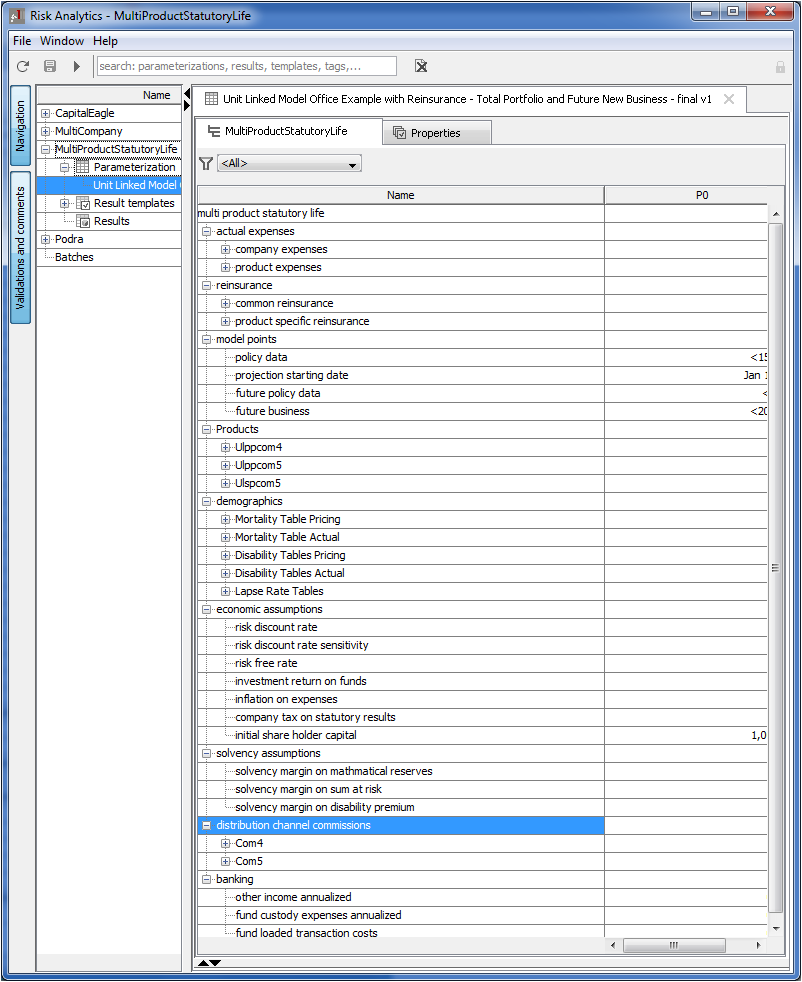
\includegraphics[scale=0.7]{images/lifep14n.png}
	\caption{The input screen for mentioned parameters}
	\label{fig:lifep14n}
\end{figure}

\subsection{Actual expenses}

The end-user can define two kinds of expenses: Overall company expenses to reflect the complete expense structure of the company (a.o.~ used in embedded value type of calculations) or product related expenses to reflect the cost-intensiveness of the different kind of products (e.g.~used for profit-testing calculations). Of course one could also define both kinds of expenses in the same model (e.g.~to capture the expenses-over-run).

Please note that all the expense definitions in this section are referring to actual expenses ("2nd order", outgoes) and do not necessarily need to be directly related to the "1st order" expenses (pricing, loadings) of the various products.

\subsubsection{Company expenses}

The company expenses are characterized by:

\begin{itemize}
	\item "company overhead expenses": Have to be entered in an absolute amount (CHF) for every month of the envisaged projection period (40 years or 480 months). However, for our model example we set all the company overhead expenses equal to 0.
  \item "apply inflation on company overhead expenses": One has to indicate whether the company expenses need to be indexed with inflation (true/false).
\end{itemize}

\subsubsection{Product expenses}

For all the defined products, expenses need to be entered separately. To add a product 'right click' on the "product expenses" tab and add a new product. Various expense types (absolute in CHF per policy, initial and administrative (i.e.~ annually recurring) as well as policy-size dependent expenses) need to be defined. We use the "ulppcom5" product as example. For the other two products similar parameters are entered.
\begin{itemize}
	\item "product": "ulppcom5" needs to be entered this is required for a clear product/expense allocation required, otherwise the program is failing).
	\item "fixed administration expenses per policy per annum": We define them at CHF 100, which in the calculation are then broken down on a monthly basis.
	\item "apply inflation on fixed administration expenses per policy": To define whether the expenses need to be indexed with inflation.
	\item "fixed initial expenses per policy": We define them at CHF 100, to capture e.g.~the initial underwriting expenses. These expenses are charged only once at the beginning.
	\item "apply inflation on fixed initial expenses per policy": To reflect whether future new business have unchanged initial expenses or whether these expenses are indexed with inflation.
	\item "variable expenses per policy": We can enter any number (by changing the "row count") of classes for policy sizes in CHF. Policy size = annual premium times premium payment duration. Depending on the policy size the "administration expenses per policy p.a.~" and "initial expenses per policy" can be defined. In our example we allocate (in addition to the above mentioned fixed expenses) for policies with a sum of premiums below CHF 200'000 administration expenses per policy of CHF 30 p.a.~and initial expenses per policy of CHF 50. For policies with a sum of premiums of CHF 200'000 or more the administration expenses are CHF 50 and the initial expenses CHF 100, cf.~figure \ref{fig:variableexpenses}\end{itemize}

\begin{figure}
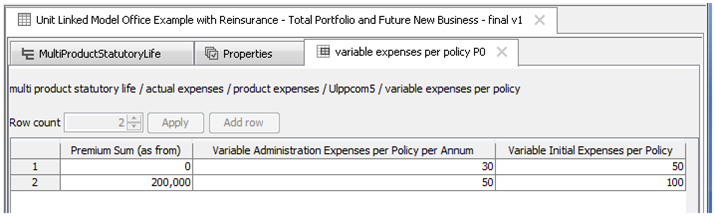
\includegraphics[scale=0.7]{images/variableexpenses.png}
	\caption{Variable expenses per policy}
	\label{fig:variableexpenses}
\end{figure}

In our example the product expenses for the other two products are very similar to "ulppcom5". However, in the real world the expenses can if necessary be entered with much more sophistication.

\subsection{Reinsurance}

Every underwriting year and currency will be separately treated (accounting series with different conditions; i.e.~with separate loss carried forward amounts and loss carried forward interest rates).

For each settlement period a profit \& loss calculation for the reinsurance is made:
\begin{itemize}
	\item It consists of
		\begin{itemize}
			\item the ceded reinsurance premium (ceded expenses and costs), plus
				\item the surrender claw-back and
				\item the extra deposit investment income.
\end{itemize}
	\item This is reduced by
		\begin{itemize}
			\item the reinsurance commissions (initial and running/recurring), and
			\item death and waiver of premium benefits (sums at risk).
		\end{itemize}
	\item The initial loss (financing via the initial reinsurance commission) will be carried forward and increased by an interest rate plus an administrative charge ("Cost and Risk Annual Supplement on Ceded Premium"). In case that we have a profit, the reinsurer pays a profit participation to the insurance company.
\end{itemize}

Please note that saving premiums as well as the surrender payments need not to be part of the above calculation in case that the funds remain with the insurance company and are not passed to the reinsurer. Furthermore, the administrative charge to the reinsurer and the loss carried forward interest rates are not directly paid by the insurance company to the reinsurer, but only notionally allowed for in the profit \& loss calculation by increasing the loss carried forward.

The end-user needs to define two kinds of parameter groups for modeling the reinsurance:
\begin{itemize}
	\item	Overall company reinsurance conditions to reflect the general treaty characteristics ("common reinsurance")
	\item 	Product specific reinsurance parameters to reflect the various reinsurance conditions (quota share, commissions, amortization/payback) on a product level.
\end{itemize}

\subsubsection{Common reinsurance}

In this section we enter the general reinsurance treaty characteristics:

\begin{itemize}
	\item "First Settlement Period Begin Date": Enter the beginning of a month date as from which on the reinsurance calculation should start. This has to be in-line with the amounts entered under "loss carried forward". We have a US-date format; i.e.~MM/DD/YY.
	\item "First Settlement Period Ends Before": This date defines the duration of the (first) settlement period. Could be e.g.~3 months after the begin date (in case of quarterly reinsurance settlements). However, in case we wish to have monthly results (as in our example), we enter one month after the begin date (format: MM/DD/YY).
	\item "First Settlement Date": Needs to be at least one day after the above end date (format: MM/DD/YY).
	\item "Settlement Interval in Months": Defines the time for interval of the settlements periods. In case of quarterly reinsurance settlements we would set 3 months.
	\item "Extra Deposit Interest Rate": The extra interest rate (p.a.~) on the reinsured funds values (saving accounts) which the insurance company will pay to the reinsurer (e.g.~to pass a part of the "kick-back" to the reinsurer). The calculation is done based on the average fund values over the specified period "Month Count for Average Fund Value" (see below). In case of quarterly settlements we might take the average fund value over the last 4 end of months (e.g.~for end 31.12., 31.1., 28.2.~and 31.3.). In our example we will, however, calculate for every month the average fund value (begin/end of month) as the basis for the calculation of the extra deposit interest.
	\item "Profit Participation": The participation (in our case we have 90\%) which the reinsurer pays to the insurance company in case that the loss carried forward becomes positive.
	\item "Loss Carried Forward Rates": Here we define for every underwriting year and currency separately the loss carried forward amounts and loss carried forward interest rates) shown in figure \ref{fig:mdplosscarriedfwrates}. In the past the insurance company in our example sold only policies during the year 2009 with a loss carried forward amount (due to the reinsurer) of CHF 147'493. The interest rate which will be used also in future accounting years for the underwriting year 2009 is 10\%. We need to specify for all the desired future years (with new business) the loss carried forward interest rate (in our example in addition to 2009 for the years 2010 to 2012; i.e.~we set the row count = 4). Of course one could have (e.g.~due to different economic situations) in the past different loss carried forward interest rates or going forward one would like to plan the new business with different loss carried forward interest rates.
	
	\item"Claw Back Percentage": In case of a lapse for a given policy the insurance company will in our example immediately amortize for this policy all the non-amortized initial reinsurance commissions (i.e.~we set the claw-back percentage = 100\%). The non-amortized reinsurance commissions are determined in the following way:
		\begin{itemize}
		\item Initial reinsurance commissions paid by the reinsurer,
			\item minus part of the initial reinsurance commissions which have been paid back by the insurance company before the lapse of the policy,
			\item	minus administration and unit expenses as well as the risk premiums ceded by the insurance company to the reinsurer,
			\item	minus extra deposit investment income ceded for this policy,
			\item	plus/minus (the balance of) the acquisition commissions which have been reallocated over time
			\item	plus the administration and unit expense running commissions paid by the reinsurer. 
		\end{itemize}
For a more detailed understanding of the parameters, see also next section.
	\item"Month Count for Average Fund Value": The calculation for the average fund value should be in-line with the settlement interval (see also above). In our example we simply assume a monthly calculation and we take the average fund value (begin/end of month; i.e.~we set the month count equal to 2).
	\item"Cost and Risk Annual Supplement on Ceded Premium": The loss carried forward will be increased by an additional administrative charge ("Cost and Risk Annual Supplement on Ceded Premium": In our example it equals 2\% of the ceded premiums).
	
\end{itemize}

\begin{figure}
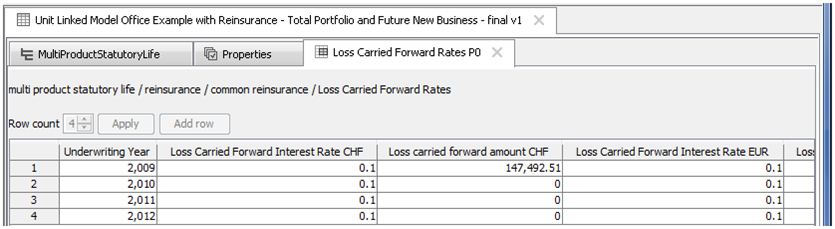
\includegraphics[scale=0.7]{images/mdplosscarriedfwrates.png}
	\caption{Loss Carried Forward Rates}
	\label{fig:mdplosscarriedfwrates}
\end{figure}

\subsubsection{Product specific reinsurance}

For all the products we need to define a separate section (use the same name as under the "products" section) and enter the reinsurance parameters, in particular: The reinsured quota share of the premium, the payment of the reinsurance acquisition (initial) commission, the reinsurance treatment of the recurring expenses as well as the amortization/payback. In case that a product is not reinsured, we simply set the quota share equal to 0. To add a product simply 'right click' on the "product specific reinsurance" tab and add a new product.

We use the "ulppcom5" product as example:
\begin{itemize}
	\item	"product": "ulppcom5" needs to be entered (this - somehow redundant information - is required for a clear product allocation).
	\item "currency": The currency of the product has to be selected.
	\item "quota share": A number in the range of 0 to 1 has to be entered. In our example we have a 50\% quota share reinsurance; i.e.~50\% of the original premium is paid to the reinsurer.
	\item "truncated policy duration": To determine the truncated sum of premiums ($SOP_{trunc}$) the policy duration (in years) is "truncated" on our example at 25 years, in case the premium payment duration is larger. If no truncated duration is required on could e.g.~enter 99 years ("lifelong"), or more.
	\item "reinsurance acquisition commission": We can define for various classes (= row count) of premium payment durations (in years) the four acquisition commission parameters A, B, C, D. In our example we only have one class (row count = 1), i.e.~for all the premium payment durations we apply the same parameters. (In our example we define the class relating to all the premium payment durations $>$ 0; i.e.~we capture all the policies because they have a premium payment duration which is greater than zero.) However one could define a row count $>$ 1 and input for various premium payment durations a separate set for the four acquisition commission parameters. (To determine which row or class of parameter set has to be applied: Premium payment duration is $\geq$ the indicated values. Of course, in this input table the listed premium payment durations need to be in strict increasing order.)
	
Lets use the following abbreviations:
\begin{itemize}
	\item $QS$:  quota share
	\item $SOP$:  sum of premiums (over the entire premium payment duration)
	\item $SOP_{trunc}$:  sum of premiums over the truncated premium payment duration
	\item $A$, $B$, $C$, $D$:  acquisition commission parameters for a given premium payment duration
\end{itemize}
We further define: 

"reinsurance acquisition commission" $=$ \\
$\max (A; \min (B; C + D/(QS \times SOP))) \times QS \times SOP_{trunc}$ \\
Given the values in our example (A=0.05 and B=C=D=0) we therefore have for all the premium payment durations a reinsurance acquisition commission of 5\% of 50\% of the truncated (at 25 years) sum of premiums. This is an illustrative and simple assumption; however, the parameters allow a more sophisticated parameterization if required.
	\item "fixed and beta expenses": To compensate for the larger administration work done by the insurance company, the reinsurer pays back to the insurance company a percentage of the fixed (kappa) and beta expenses he receives\footnote{The reinsurer receives the quota share of the original fixed (kappa) and beta expense loadings.}.{}
The paid-back percentage is equal to: $1 - \min (A; B + (QS \times SOP)/C)$, where A, B and C are the parameters for the reinsurance expenses. QS and SOP defined as above. The Parameter C is a kind of calibration for the SOP and needs always to be set $> 0$ (otherwise we would have an error due to a division by 0), also in the case where QS is equal to 0\%. Please note that for the "fixed and beta expenses" parameters the row count has always to be equal to 1.
Given the values in our example (A=B=0.75 and C=1) the reinsurer therefore pays back 25\% of the received fixed (kappa) and beta expenses to the insurance company. 
	\item "amortization of acquisition commission in years": This parameters defines the "acquisition commission reallocation over time". The policyholder has to amortize the charged acquisition commission over a given period (in our example: 10 years; see later in the section \ref{sec:lifeproducts} about "products"). However, the amortization of the reinsurance acquisition commission does not necessarily need to be done over the same period. In our example we have defined 8 years, i.e.~we have to reallocate in a different cash flow pattern the amortization of the acquisition commission and the insurance company will pay 1.25 (=10/8) of the original acquisition commission loading times the quota share to reinsurer. However, one could also imagine another example where the amortization of the acquisition commission for the reinsurance has a longer duration than the amortization in the original product. In such a case the reinsurer would pay-back in a first phase a part of the received acquisition commission to the insurance company. Please note that the calculation of the amortization patterns assumes that the sum of the original acquisition commission loadings (paid by the policyholder) times the quota share is equal to the sum of the loadings of the reinsurance acquisition commission.
\end{itemize}

For the other two products similar parameters are entered. Note please that there is no reinsurance for the single premium product "ulspcom5" (quota share = 0).

\subsection{Model points and projection starting date}
\subsubsection{Policy data}

In this section we describe the existing portfolio: In our example the portfolio consists of 100 policies which have been sold in 2009. The so-called model point (one line in the policy data table) represents one sold policy. We need to enter the following policyholders' information, which in general can (automatically) be extracted from the administration system:

\begin{itemize}
	\item "Policy \#": This could be a number to identify the policy.
	\item "Product": The identifier used in the products section to denominate the product.
	\item "Annual Premium": The amount of the gross annual premium or of the single premium paid by the policyholder. (If 0 is entered, the policy is not considered.)
	\item "Alpha": represents the acquisition commission loading paid by the policyholder. In our example for all the policies $\alpha$ is equal to 5\% of the present value of premiums or of the sum of premiums. However, because in the life insurance model this parameter does not depend from the product description, one could also imagine that the policies could have variable acquisition commission loadings.
	\item "Installments pa": The annual installments, e.g.~monthly (12), quarterly (4), half-yearly (2) or annual (1).
	\item "Gender": 'male' or 'female'.
	\item "Birthdate": In the format YYYY-MM-DD.
	\item "Policy Inception Date": In the format YYYY-MM-DD.
	\item "Premium Payment Duration [Years]": The original payment duration in the policy contract. e.g.~for single premium the premium payment duration is equal to 1.
	\item "Policy Duration [Years]": The original policy duration in the contract.
	\item "Risk Sum (relative)": In case of death of the policyholder the funds value (mathematical reserves) plus the "risk sum (relative)" will be paid-out. The "risk sum (relative)" is expressed as a factor of the sum of premiums.
	\item "Minimal Death Benefit": An absolute amount (in CHF), which will at least be paid-out in case of death of the policyholder. In case that the funds value (mathematical reserves) is larger than the minimal death benefit, only the funds value will be paid out. The sum at risk is equal to the difference ($\geq 0$) between the 'minimal death benefit' and the funds value (mathematical reserves).
	\item "Waiver of Premium Covered": 'false' or 'true'.
	\item "Waiver of Premium Waiting Delay": We have in our disability tables values for 6, 12 and 24 months of waiting periods. In case that no waiver of premium is covered, set this value equal to 0. The sum at risk is calculated as the risk free discounted value of premiums after the waiting period.
	\item "Mathematical Reserves": The actual reserves are usually extracted from the administration system and calculated for date as per the projection start date (in our example as per 31.12.2009).

\end{itemize}

\subsubsection{Projection starting date}

In our example we define the begin of the first period with 1.1.2010 (Input: DD/MM/YYYY). We have an existing portfolio as per 31.12.2009 and we assume for three years going forward future new business (i.e.~for 2010 -- 2012).

\subsubsection{Future policy data}

With the row count we define the number of future model points. In our example we have three model points; i.e.~one for each of the three products. This describes the kind of policies sold in future. (For this open available life model, the input (= row count) is limited to 20 model points.) Of course, one could also define several and different policies (model points) for one product to capture and reflect the characteristics of the product for some particular parameters:

\begin{itemize}
	\item	"Model Points": The model points are denoted with MP1, MP2 and MP3, etc.
	\item	"Product": The identifier used in the products section to denominate the product.
	\item	"Annual Premium": The amount of the gross annual premium paid by the policyholder.
	\item	"Alpha": $\alpha$ represents the acquisition commission loading paid by the policyholder. In our example for all the policies $\alpha$ it is equal to 5\% of the present value of premiums or of the sum of premiums. However, because in the life insurance model this parameter does not depend from the product description, one could also imagine that the policies could have variable acquisition commission loadings.
	\item	"Installments pa": The annual installments, e.g.~monthly (12), quarterly (4), half-yearly (2) or annual (1).
	\item	"Gender": 'male' or 'female'.
	\item	"Age": Age of the policyholder in years when the policy will be sold (in future).
	\item	"Premium Payment Duration [Years]": The original payment duration in the policy contract. e.g.~for single premium the premium payment duration is set equal to 1.
	\item	"Policy Duration [Years]": The original policy duration in the contract.
	\item	"Risk Sum (relative)": In case of death of the policyholder the funds value (mathematical reserves) plus the "risk sum (relative)" will be paid-out. The "risk sum (relative)" is expressed as a factor of the sum of premiums.
	\item	"Minimal Death Benefit": An absolute amount (in CHF), which will at least be paid-out in case of death of the policyholder. In case that the funds value (mathematical reserves) is larger than the minimal death benefit, only the funds value will be paid out. The sum at risk is equal to the difference ($\geq 0$) between the 'minimal death benefit' and the funds value (mathematical reserves).
	\item	"Waiver of Premium Covered": 'false' or 'true'.
	\item	"Waiver of Premium Waiting Delay": We have in our disability tables values for 6, 12 and 24 months of waiting periods. In case that no waiver of premium is covered, set this value equal to 0. The sum at risk is calculated as the risk free discounted value of premiums after the waiting period.
\end{itemize}

Of course, policies which are sold going forward do not have mathematical reserves to be considered at the beginning of the projection (as we have in the existing portfolio -- see above). The model points for the future policy data should represent in a reasonable way the characteristics (types) of the policies which are sold in future. The number of sold policies (model points) is entered in the next session.

\subsubsection{Products} %was 'Future business' 

The number of sold policies need to be defined by starting in period 0 (this corresponds to the starting of the projection; i.e.~to January 2010 in our example): Month by month, for up to 120 periods or 10 years the number of sold policies (as defined above by the model points - future policy data) can be entered. (Please note that in the open available life model, the row and column counts can not be changed.)

For the next 3 years we expect in our example total (future) sales of 900 policies for the three products (model points): 200 policies in 2010, 300 policies in 2011 and 400 policies in 2012. With the existing portfolio we therefore capture and model 1'000 policies in total. This is illustrated in figure \ref{fig:mdpfuturebusiness}. 

\begin{figure}
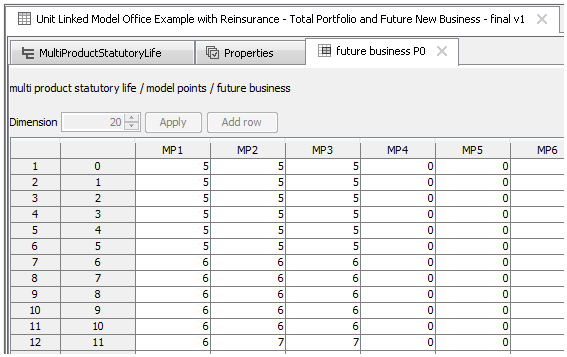
\includegraphics[scale=0.7]{images/mdpfuturebusiness.png}
	\caption{Future business - entering number of sold policies (by model points and months)}
	\label{fig:mdpfuturebusiness}
\end{figure}

\section{Input parameters}\label{sec:lifeproducts}

The following parameters are the core input to describe the products, through these characteristics of the unit-linked policies. Combined to these unit-linked products one could also have death benefits and waiver of premium insurance. These coverages are not further described here; they are captured on a per policy basis in the policy data description (see above). However, the costs for these coverages are either charged to the premium or to the actual funds values (saving account or component of the product).

One can define as many products as desired, also by using meaningful, internal names: We describe subsequently the parameters of the (first) product "ulppcom5" (periodic premium payment and linked to commission payment rule "com5"):

\begin{itemize}
	\item	"Products": 'Right click' on "products" and add a new product by entering the desired name; in our example "ulppcom5".
	\item	"currency": Choose the desired currency
\end{itemize}

\subsubsection{Acquisition expenses alpha ($\alpha$):}

\begin{itemize}
	\item "alpha calculation base": The calculation base for the acquisition commission loading $\alpha$ (which is defined in the model points - policy data section) could either be the present value of premiums $PV$ or of the sum of premiums $SOP$.
	\item "technical interest rate for present value of premium": The technical interest rate $i$ which is used to calculate the present value of premiums is in our example 1.75\%.
The total acquisition commissions AC charged to the policyholder are therefore: \\

$AC = \alpha \times PV$ or $AC = \alpha \times SOP$\\

The $AC$ are amortized over a duration $m_1$ or $m_2$ depending on various conditions (for the policy duration $n$ and for the annual premium $AP$):
	\item "alpha threshold policy duration in years": This is denoted with $T(n)$ and is in our example 10 years.
	\item "alpha threshold annual premium": This is named with $T(AP)$ and is in our example CHF 1'000.
	\item "alpha amortization time in years min": This is denoted with $m_1$ and is in our example 10 years.
	\item "alpha amortization time in years max": This is denoted with $m_2$ and is in our example 10 years.
With $t$ we denote the actual policy year (from 1 to $n$) and with $\mu$ the number of  the annual installments [e.g.~monthly (12), quarterly (4), half-yearly (2) or annual (1)].


The acquisition commissions $AC_t$ charged in year $t$ (charged against the actual
premium payment) are then defined by:
\begin{eqnarray*}
AC_t & = & \left\{\begin{array}{rl}
\displaystyle{\frac{AC}{u\cdot\ddot{a}^{(u)}_{\overline{m_1}\!|}} }& \mbox{if
}[n<T(n)\mbox{ or
}AP>T(AP)]\mbox{ and }t\leq m_1\\\\
\displaystyle{\frac{AC}{u\cdot\ddot{a}^{(u)}_{\overline{m_2}\!|}} }& \mbox{if
}[n\geq T(n)\mbox{ and
}AP\leq T(AP)]\mbox{ and }t\leq m_2\\\\
0 & \mbox{otherwise}
\end{array}\right.
\end{eqnarray*}
and where
\begin{equation*}
\ddot{a}^{(u)}_{\overline{t}\!|}\,=\,\frac{1-v^t}{d^{(u)}}\,,\quad
v\,=\,\frac{1}{1+i}\,,\,\,\,\mbox{ and }\,\,\,d^{(u)}\,=\,u\cdot[1-(1+i)^{-1/u}]\,.
\end{equation*}

With $i$ we denote the technical interest rate. In our example we have simplified assumptions where the AC are always amortized over a fixed period of 10 years ($m_1 = m_2 = 10$). The threshold for the annual premium $T(AP)$ does basically not play a role in the above formulae. Finally, the product design makes only sense if the policy duration is at least 10 years (i.e.~no policies with a policy duration $n < 10$ should be sold).
\end{itemize}

\subsubsection{Collection expenses beta ($\beta$):}

During the premium payment period the beta expenses $\beta$ in proportion to the periodic premium are charged to the policyholder. With the 5 beta parameters (A, B, C, D and E) various cost structures can be modeled. We define: 
$\beta = \min (A + \max (B;(n-C) \times D); E)$, where $n$ is the policy duration. In our example we have beta expenses varying between 7\% and 8\% of the premium:
\begin{itemize}
	\item "beta a": Is set equal to 0.07
	\item "beta b": Is set equal to 0
	\item "beta c": Is set equal to 15
	\item "beta d": Is set equal to 0.001
	\item "beta e": Is set equal to 0.08
\end{itemize}

\subsubsection{Proportional administration expenses gamma ($\gamma$):}

During the entire policy duration the gamma expenses $\gamma$ in proportion to the funds value are charged (by reducing the funds value respectively the mathematical reserves).
In our example we charge 0.05\% p.a.~of the funds value.
\begin{itemize}
	\item "gamma1 of mathematical reserves": Is set equal to 0.0005 p.a.~
	\item "gamma2 of mathematical reserves": Is set equal to 0 p.a.~
\end{itemize}
We have two gamma parameters. With gamma2 one could e.g.~model a bonus parameter or a kick-back refund to the policyholder by setting a negative parameter (negative charge).
Please note that the gamma expenses are calculated at the beginning of every month and charged on a monthly basis; i.e.~the above gamma parameters are divided by 12.

\subsubsection{Fixed administration expenses kappa ($\kappa$):}

During the entire policy duration the (annual) kappa expenses $\kappa$ in CHF are charged to the policyholder at the beginning of every month (i.e.~1/12). With the 5 (periodic premium products) respectively 6 (single premium products) kappa parameters (A, B, C, D, E and F) various cost structures can be modeled.

We define for the periodic premium products: 
$\kappa = \min (A + \max (B;(n-C) \times D); E)$, where $n$ is the policy duration.
And for the single premium products (i.e.~premium payment duration = 1 year):
$\kappa = \min (A + \max (B;(n \times{{SP}/{F}}-C) \times D); E)$, where $SP$ is the single premium.
In our example we have kappa expenses varying between CHF 50 and CHF 100 p.a.~:
\begin{itemize}
	\item "kappa a": Is set equal to 50
	\item "kappa b": Is set equal to 0
	\item "kappa c": Is set equal to 15
	\item "kappa d": Is set equal to 2.50
	\item "kappa e": Is set equal to 100
	\item "kappa f": Is set equal to 0 (as it is n/a for the "ulppcom5" product)
\end{itemize}

\subsubsection{Other parameters:}

\begin{itemize}
	\item "surrender charge of funds": In case of a surrender a penalty (charge) in proportion to the funds value is charged to the policyholder depending on the elapsed time. A variable scale can be entered. In our example we have a monthly linearly falling charge (from 100\% to 0\%) over the first 5 policy years. However, one could also define a flat (constant) surrender percentage over the entire policy duration.
	\item "mortality table pricing": The desired mortality table has to be selected. The risk premium (1/12 of the q(x)) is charged at the beginning of every month (reduction of policyholders' funds).
	\item "mortality table actual": The desired mortality table has to be selected.
	\item "waiver of premium pricing": The desired waiver of premium table has to be selected. The risk premium (1/12 of the i(x)) is charged at the beginning of every month (reduction of policyholders' funds).
	\item "waiver of premium actual": The desired waiver of premium table has to be selected.
	\item "lapses": The desired lapse table has to be selected.
	\item "distribution channel selection": The desired commission payment type or "scale" has to be selected (according to the required distribution channel remuneration, etc.) 
\end{itemize}

For the other two products similar parameters are entered.

\subsection{Demographics}

\subsubsection{Mortality}

Two mortality tables have been defined, for pricing purposes and for actual outcomes:	
\begin{itemize}
	\item "bfs mort19982003": Derived from BFS-data (Bundesamt fuer Statistik) a pricing mortality table with ultimate q(x) for male and q(y) for female has been entered (to import the data into PillarOne: simply use copy/paste from Excel).
	\item "bfs actual": The mortality table with the actual values has been defined as 80\% of the pricing mortality table.
\end{itemize}
For pricing purposes the risk premium charges are determined according to the "age last birthday". For actual valuation purposes the mortality is calculated by interpolating (i.e.~"exact").

The end-user can define the size of the table and at which age the table should start. There are no limits with respect to the number of mortality tables (and also other tables, e.g.~for disability, lapses, commissions, etc.) one would like to define. To create a new table simply 'right click' on "mortality table" tab and add a new table. For example one could define a different mortality table for every product.

\subsubsection{Disability}

Two disability tables have been defined, for pricing purposes and for actual outcomes (as they are derived from the "Invaliditaetsstatistik 1996/2000 in der schweizerischen Kollektivlebensversicherung", SAV Bulletin 2/2004):
\begin{itemize}
	\item "waiver of premium": Disability table for pricing purposes for both gender ($i(x)$ and $i(y)$) and 3 waiting periods of 6, 12 and 24 months, cf.~figure \ref{fig:mdpwaiverofpremium}
	\item "waiver of premium actual": This disability table has been calculated as 80\% of the pricing disability table.
\end{itemize}

\begin{figure}
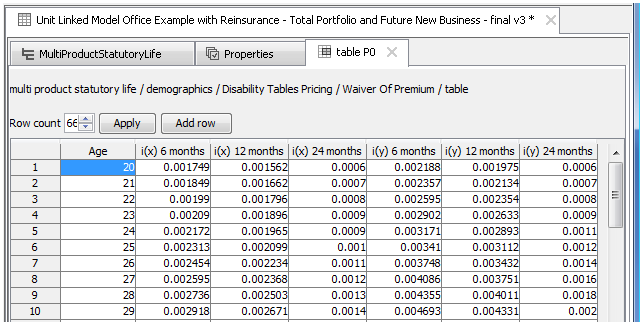
\includegraphics[scale=0.7]{images/mdpwaiverofpremium.png}
	\caption{Waiver of premium table for pricing}
	\label{fig:mdpwaiverofpremium}
\end{figure}

For pricing purposes the risk premium charges are determined according to the "age last birthday". For actual valuation purposes the disability rate is calculated by interpolating (i.e.~"exact").

The end-user can define the size of the table and at which age the table should start. There are no limits with respect to the number of disability tables.

Disability is modeled as an event terminating the policy, like death or surrender. In case of disability, the policyholder receives his savings (funds value) at end of month plus the risk free discounted value of premiums after the waiting period. No reactivations are modeled.

\subsubsection{Lapses}

Various lapse rate tables have been defined, e.g.:
\begin{itemize}
	\item "lapse rate1" (the 'main' table in our example for the periodic premium products): To reflect that in the 6th year the lapse rate is increasing again for the periodic premiums because of the discontinuation of the surrender charge (after 5 years).
	\item "lapse rate2": With continuing falling lapse rates for the single premium product.
\end{itemize}
Various other tables have been created for testing purposes (for example for calculation with one policy): e.g.~to simulate "no lapse", "surrender in year2" or "surrender in year5".

\subsection{Economic assumptions}

Further, simple parameters (not e.g.~interest curves, remain constant over the entire projection period) can be entered in the economic assumptions section:
\begin{itemize}
	\item "risk discount rate": 7.5\%
\item "risk discount rate sensitivity": not used
\item "risk free rate": 1.5\%
\item "investment return on funds": 5.0\%
\item "inflation on expenses": 1.0\%
\item "company tax on statutory results": 25.0\%
\item "initial share holder capital": CHF 1'000'000
\end{itemize}

\subsection{Solvency assumptions}

Only the capital requirements under the Solvency I regime are modeled in this life insurance PillarOne model to compute the minimal solvency capital which is locked-in. In our example we set 100\% of the standard solvency parameters:
\begin{itemize}
	\item "solvency margin on mathematical reserves": 1.0\%
	\item "solvency margin on sum at risk": 0.3\%
	\item "solvency margin on disability premium": 20\% of the annualized disability (waiver of premiums) risk premiums
\end{itemize}
The values are calculated at the end of every month.

\subsection{Distribution channel commissions}

Various distribution channels can be defined: 'Right click' on "distribution channel commissions" and add a new commission section by entering the desired name; in our example "com5".
For "com5" we define the following parameters:

\begin{itemize}
	\item "acquisition commission": In our example the insurance company pays an acquisition commission of 5.0\% of the calculation base. The calculation base could either be the present value of premiums or of the sum of premiums. The acquisition commission is fully paid out in the month when the policy is sold (i.e.~upfront at the policy inception date).
\item "acquisition commission base": In our example we select "sum of premiums" as calculation base.
\item "discount rate for present value of premiums": The interest rate which is used to calculate the above mentioned present value of premiums. In our example we do not use it.
\item "apply max duration": We have to select whether or not the policy duration is capped (or 'truncated').
\item "max duration in year": In our example the policy duration will be capped at a maximum of 25 years.
\item "portfolio commission annualized": In our example the insurance company also pays out a portfolio commission of 0.05\% p.a.~of the 'mathematical reserves' ("portfolio commission base"). The payment is done on a monthly basis (i.e.~1/12).
\item "portfolio commission base": Is the 'mathematical reserves' (no selection possibility).
\item "claw back share": In case of a surrender the acquisition commission has to be refunded ("claw-back") by the distribution channel (agent) to the insurance company ("non-amortized" part of the initial or acquisition commissions due by the agent). A variable (row count) claw-back scale can be entered. In our example we have a linearly falling claw-back share within the first 3 policy years (or 36 months). Only after the first 3 years the acquisition commissions are fully earned.
\item "shortfall of claw back": Additionally we can define a shortfall of the claw-back payment; i.e.~when the distribution channel fails to pay back the due part of the acquisition commissions. A probability table for the shortfall of claw-back can be entered. (Variable size of the table is being defined with the row count.) In our example we assume a general (flat: row count = 1) probability of shortfall of 2.5\% of the claw-back share for all the months.
\end{itemize}

For the distribution channel commission "com4" we have the same input except for the "acquisition commission": 4.0\%. This could be justified if e.g.~the administrative work done by the insurance company is varying between the different distribution channels or for various products.

\subsection{Banking}

The banking transactions are creating additional expenses or other income. We have three types of parameters which can be used to simulate these effects:
\begin{itemize}
	\item "other income annualized" ("kick-back"): In some circumstances the banks are paying a fee to the insurance company ("kick-back") to compensate for the various investment processes. In our example we assume that the insurance company will get 0.25\% p.a.~(or 25 bp) of the funds value. The model, however, calculates and accrues the 'other income' on a monthly basis (i.e.~1/12).
\item "fund custody expenses annualized": In our example we assume for the insurance company fund custody expenses of 0.05\% p.a.~of the funds value. These expenses are also calculated and accrued on a monthly basis (i.e.~1/12).
\item "fund loaded transaction costs": Finally, in our example, we also have modeled transaction costs of 0.25\% of the net buy-sell amount (monthly) which the insurance company will have to pay (0.25\% of the monthly change in reserves).
\end{itemize}

\section{Running calculations}

For doing the calculations there are a few parameters which need to be entered. Usually the simulation settings are defined by the newest version of the parameters as illustrated in figure \ref{lifecalculation}:

\begin{figure}
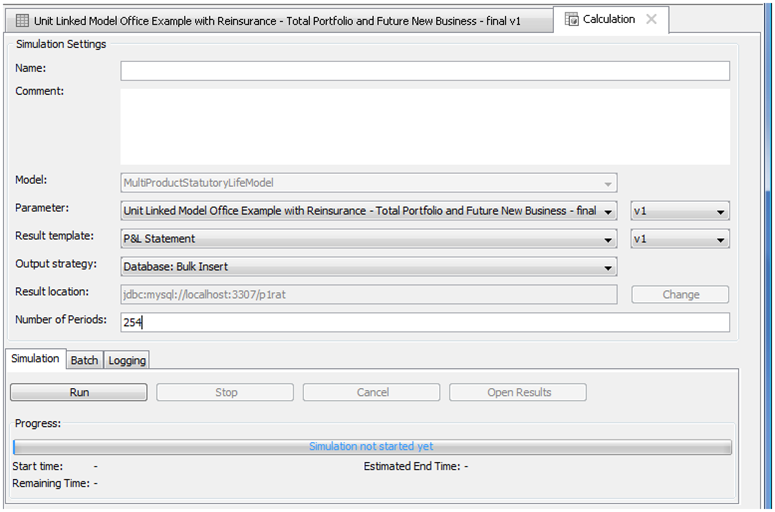
\includegraphics[scale=0.7]{images/lifecalculation.png}
	\caption{Calculation settings}
	\label{fig:lifecalculation}
\end{figure}

Important is -- in addition to the version of the parameters -- the definition of the duration of the projection (simulation) to start the calculation of the projections:

\subsubsection{"Number of Periods" (in months):}
We do ("only") one run respectively a projection with 254 periods or months (because of exporting the results with "copy/paste" into the old Excel which has only 256 columns). This corresponds to a projection period of over 21 years. However, one could do without problems also projections over 40 years or 480 periods (the Excel 2007 version has enough columns to import this directly).

One could also prepare several runs and start them on a batch-basis (e.g.~over night) to do various calculations and analysis with no further input and manual interventions.

The run times need to be analyzed for models with larger portfolios. However, our small portfolio and calculation/projection over 21 years needed approximately 15 seconds of computation time on an older laptop PC.


\section{Results and output presentation}

In this section we comment the results which are presented with a standard Profit \& Loss grid for the statutory net income and some portfolio information (balance sheet, key figures). The results can easily be imported into an Excel spreadsheet ("copy/paste"). The results are illustrated in figure \ref{liferesult}

\begin{figure}
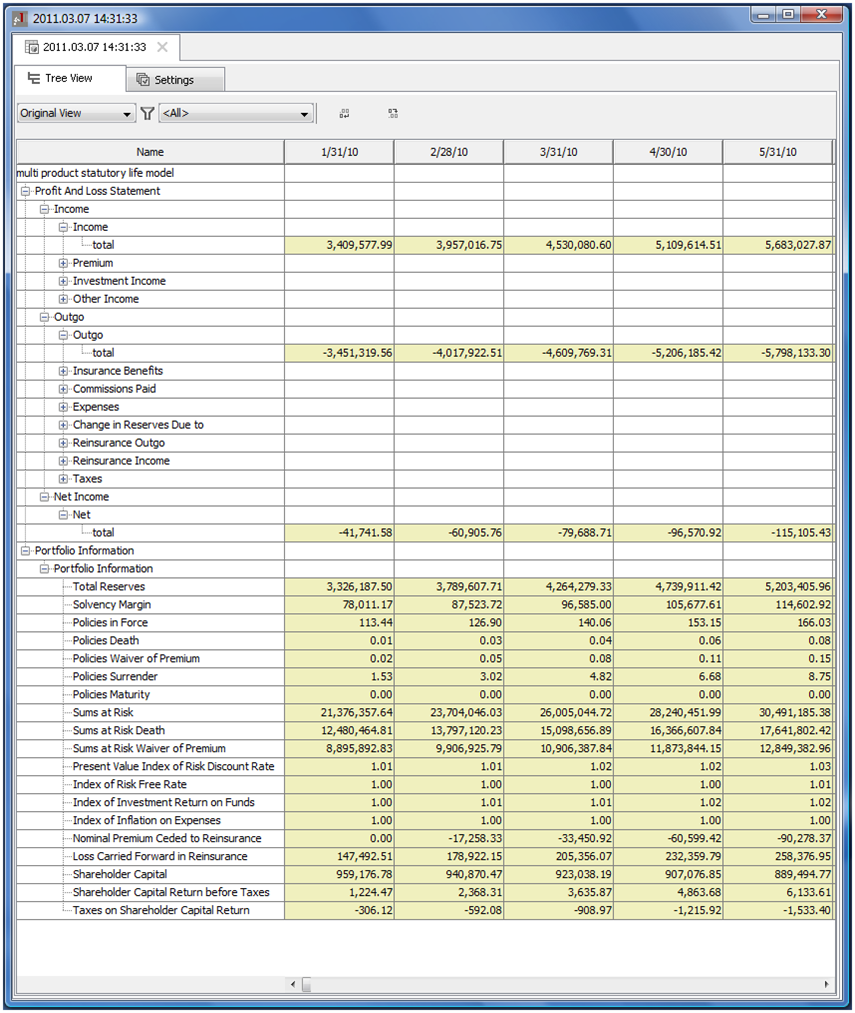
\includegraphics[scale=0.7]{images/liferesult.png}
	\caption{Results of the calculations (projections)}
	\label{fig:liferesult}
\end{figure}

The various positions are presented on a monthly basis; i.e.~we calculate and see monthly results. During the year, the data is accumulated (i.e.~the model shows "year-to-date" information) and at the beginning of a new year the data start again from zero. One can therefore easily read from the output the quarterly or half-yearly information and of course the year-end (December columns). One can 'click' (drill-down) on the various profit \& loss items and in general one receives a detailed, technical split ("internal view") of the elements. Positive figures denote an income for the insurance company, negative figures an outgo. Therefore a positive net income is a profit and a negative net income is a loss.

\subsection{Income}

The income consists of premiums, investment and other revenues.

\subsubsection{Premium}
The total premium is directly segregated (presented) into the following (technical) elements:
\begin{itemize}
	\item saving premium: Paid premium less the alpha, beta and kappa expenses.
	\item alpha: The acquisition commissions which are charged to the policyholders.
	\item beta: The beta expenses (collection expenses) which are charged to the policyholders.
	\item kappa: The fixed administration expenses (kappa) which are charged to the policyholders.
\end{itemize}

\subsubsection{Investment income}
The total investment income is equal to the investment income on the policyholders' funds:
\begin{itemize}
	\item ph funds: Investment income on the policyholders' funds.
  \item sh assets and claims reserves: These amounts are not calculated (Investment income on shareholders' funds is not presented in the profit \& loss statement; see also comment under net income).
\end{itemize}

\subsubsection{Other income}
The total other income includes the portfolio transfer:
\begin{itemize}
	\item other: Other income respectively "kick-back" paid by banks.
	\item portfolio transfer: In the first month of the projection the mathematical reserves at the start of the projection.
\end{itemize}


\subsection{Outgo}
The outgo consists of insurance benefits, commissions paid, expenses, change in reserves, reinsurance outgo/income and taxes. These elements are explained in the following sections.

\subsubsection{Insurance benefits}
The total insurance benefits are the amounts paid to the policyholders. The payments are financed by reducing the reserves (policyholders' funds) or by the risk premium payments (which are also financed at the beginning of every month by reducing the policyholders' funds).
\begin{itemize}
	\item death: Payment in case of death according to the actual mortality table.
	\item waiver of premium: This (disability) is modeled as an event terminating the policy, similar to a surrender. In case of disability, the policyholder receives his savings at end of month plus the risk free discounted value of premiums after the waiting period.
	\item surrender: Surrender benefit which is paid to policyholders (please note that the surrender charge is reduced from the policyholders' funds and flows as an income to the insurance company).
	\item terminal benefit or maturity payment: The funds value which will be paid to policyholders when the policies expire.
\end{itemize}

\subsubsection{Commissions paid}

The commissions paid relate to the distribution channel and include all the commission types plus the claw-back less the shortfall of the claw-back:
\begin{itemize}
	\item acquisition: Initial commission payment to the distribution channel in the month of the policy inception.
	\item portfolio: The ongoing portfolio commission payments.
	\item nominal clawback: The "non-amortized" initial or acquisition commissions ("claw-back") which are due from the distribution channel in case of a lapse. This is an income for the insurance company and has a positive sign.
	\item clawback shortfall: The shortfall of the above.
\end{itemize}

\subsubsection{Expenses}
The total expenses are the actual expenses ("2nd order") and include company and product expenses as well as the banking costs:
\begin{itemize}
	\item company overhead
	\item fixed initial per policy
	\item fixed admin per policy
	\item variable initial per policy
	\item variable admin per policy
	\item banking transaction costs
	\item banking custody expenses
\end{itemize}

\subsubsection{Change in reserves}
The total change in reserves consists in negative (outgo) and positive (income) items for the insurance company:
\begin{itemize}
	\item saving premium: Same amount (but with negative sign) as the saving premium under income.
	\item kappa: Fixed administration expenses ("1st order"), positive amount (part of the kappa expenses which cannot be deducted from the premiums, e.g.~for single premium products).
	\item gamma1: Proportional administration expenses ("1st order"), positive amount.
	\item gamma2: Proportional administration expenses ("1st order"), positive amount.
	\item risk premium for death: Risk premium charged to policyholders ("1st order").
	\item risk premium for waiver of premium: Risk premium charged to policyholders ("1st order").
	\item investment income: Corresponds to the investment income on the policyholders' funds (see above, but with negative sign).
	\item death benefit: Reserves which become free due to deaths of policyholders (positive amount).
	\item surrender benefit: Reserves which become free due to surrenders of policyholders (positive amount).
	\item waiver of premium benefit: Reserves which become free due to disability of policyholders (positive amount).
	\item terminal benefit or maturity payment: Reserves which become free due to maturity of the policies (positive amount).
	\item portfolio transfer: Corresponds in the first month of the projection to the mathematical reserves at the start of the projection (see other income above, but with negative sign).
\end{itemize}

\subsubsection{Reinsurance outgo}
The reinsurance cash flow is generally presented under outgo with two items, a negative (outgo) and a positive (income) one. Usually, on a longer term the reinsurance is an expenditure which the life insurance company has. The reinsurance outgo and income positions are calculated at the end of each month but presented in the output at the beginning of following month. In case one would need a precise monthly closing one would need to manually include the reinsurance positions of the subsequent month to have a "clean" (correct) accrual with a corresponding tax adjustment (this can easily be done in Excel). The reinsurance outgo includes the following positions (calculated according or in proportion to the quota share of the various products):
\begin{itemize}
	\item premium risk death ceded
	\item premium risk disability ceded
	\item premium alpha ceded
	\item premium unit expenses ceded [i.e.~fixed administration expenses (kappa)]
	\item premium admin expenses ceded [i.e.~beta (collection) expenses] 
	\item surrender clawback
	\item extra deposit investment income
\end{itemize}

\subsubsection{Reinsurance income}
The reinsurance income includes the following positions:
\begin{itemize}
	\item reinsurance commissions
	\item acquisition commission reallocation over time: The acquisition commission is reallocated over time according to the "amortization of acquisition commission in years" parameter (see also section "Product specific reinsurance"). This item could have a positive or negative sign.
	\item admin running commissions [i.e.~beta (collection) expenses]: Reinsurance company pays back to the reinsurance company a part of the expenses it receives.
	\item unit running commissions [i.e.~fixed administration expenses (kappa)]: Reinsurance company pays back to the reinsurance company a part of the expenses it receives
	\item death benefits in excess of savings
	\item waiver of premium benefits
	\item profit participation
\end{itemize}

\subsubsection{Taxes}
Taxes are calculated as a simple percentage based on all the above income less outgo positions.

\subsection{Net income}
The net income only deals with the policyholders' funds and not with the shareholders' funds (which are included under 'portfolio information'). It is the sum of the income minus the outgo.

\subsection{Portfolio information}
Following portfolio information (a.o.~balance sheet elements) and/or key figures are calculated at the end of each month:
\begin{itemize}
	\item total reserves
	\item solvency margin
	\item policies in force: Total number of policies.
	\item policies death: Number of policyholders who died.
	\item policies waiver of premium: Number of policyholders who became disabled.
	\item policies surrender: Number of policyholders who surrendered their policy.
	\item policies maturity: Number of policies which came to maturity.
	\item sums at risk: Total sums of death plus disability (waiver of premium)
	\item sums at risk death
	\item sums at risk waiver of premium: Risk free discounted value of premiums after the waiting period
	\item present value index of risk discount rate
	\item index of risk free rate
	\item index of investment return on funds
	\item index of inflation on expenses
	\item nominal premium ceded to reinsurance
	\item loss carried forward in reinsurance: Includes the 'cost and risk annual supplement on ceded premium'.
	\item shareholder capital: Is equal to the 'shareholder capital' of the previous period plus the 'shareholder capital return before taxes' minus the 'taxes on shareholder capital return'.
	\item shareholder capital return before taxes
	\item taxes on shareholder capital return
\end{itemize}

With the last three lines (above) one could also approximately build-up a financial position of the shareholder and e.g.~compare this with the required solvency margin. In our example we see that between March 2012 and May 2013 the company would have enough liquidity but the required Solvency I margin would not be fulfilled.

\subsection{Subsequent treatment}
Separate (batch) calculations could be set-up and done for a single policy (profit testing purposes), a specific product, a sub-portfolio or the entire business of the life insurance office. The various results of PillarOne can easily be imported into an Excel spreadsheet ("copy/paste")\footnote{Please note that: Excel 2003 has only 256 columns, which correspond to number of projected months (runs) if one would simply like to "copy/paste" the PillarOne results into Excel.}.{}

With the grouping function and an Excel-template sheet the monthly PillarOne results could then easily be presented on e.g.~an annual or a quarterly basis.

Subsequent treatment could e.g.~be the present value calculations of the cash flows (value of business in force) or cost of capital derivation (cost of locking-in), etc.

\section[Future development]{Future development of the life insurance PillarOne cash flow model}\label{sec:lifeoutlook}
We hope to receive feedback and input from the users of this life insurance PillarOne model.

We could further develop this first building block on various areas. Here are some high-level ideas:
\begin{itemize}
	\item Extend this model for including traditional life insurance products (not only unit-linked)
	\item Model assets and asset-dependent dynamics of life insurance business (e.g.~dynamic lapse rates, bonus participation, investment strategies)
	\item Enhance to do stochastic simulations (to do TVOG, MCEV, etc. calculations)
	\item Perform dynamic ALM-analysis, economic capital and solvency II calculations, etc.
\end{itemize}

